\documentclass[a4paper,12pt]{article}
\usepackage[T2A]{fontenc}			% кодировка
\usepackage[utf8]{inputenc}
\usepackage[english]{babel}

\usepackage{geometry}     
              % задание полей текста
\geometry{left=15mm,right=15mm,top=20mm,bottom=20mm}
\usepackage{listings}
\usepackage{cmap}					% поиск в PDF
\usepackage[T2A]{fontenc}			% кодировка
\usepackage[utf8]{inputenc}
\usepackage[english]{babel}	% локализация и переносы
\usepackage{natbib}

\usepackage{graphicx}
\graphicspath{{pix/}}

\usepackage{xcolor}
\usepackage{hyperref}
\usepackage{amsmath}
\usepackage{amssymb}
\usepackage{enumerate}
\usepackage{dsfont}
\usepackage{mathrsfs}
\usepackage[normalem]{ulem}

\setlength\parindent{0pt}

\sloppy                                    % строго соблюдать границы текста
\linespread{1.3}                           % коэффициент межстрочного интервала
\setlength{\parskip}{0.5em}                % вертик. интервал между абзацами

\setcounter{secnumdepth}{0}                % отключение нумерации разделов
\binoppenalty=1000                         % уменьшение переносов в формулах
\usepackage[T2A]{fontenc}			% кодировка
\usepackage[utf8]{inputenc}
\usepackage[english]{babel}	% локализация и переносы

\usepackage{graphicx}

\setlength\parindent{0pt}

\sloppy                                    % строго соблюдать границы текста
\linespread{1.3}                           % коэффициент межстрочного интервала
\setlength{\parskip}{0.5em}                % вертик. интервал между абзацами

\usepackage{lipsum}
\usepackage{easy-todo} % Добавление задач с помощью \todo{}
\usepackage{csquotes} % Для "правильных" кавычек

\usepackage[activate={true,nocompatibility},
	final,
	tracking=true,
	kerning=true,
	expansion=true,
	spacing=true,
	factor=1050,
	stretch=25,
	shrink=10]{microtype} % Für die Feineinstellung der Zeichensetzung.
\usepackage{booktabs}
\usepackage{appendix}
\usepackage[rflt]{floatflt}
\usepackage{fancyvrb}
% \usepackage[hidelinks]{hyperref} % Klickbare aber nicht markierte Links im PDF
\usepackage{setspace}
% \usepackage{fancyhdr} % Für schönere Kopf-/Fußzeilen und Fußnoten.
% \usepackage[right=4 cm, left=2.5 cm, top=2.5 cm, bottom=3 cm]{geometry} % Seitenränder
\usepackage{pbox}
\usepackage{tabulary}

\hypersetup{
    pdfstartview=FitH,
    colorlinks=true,
    linkcolor=blue,
    filecolor=magenta,      
    urlcolor=cyan,
}

\usepackage{titleps}                       % колонтитулы

\newpagestyle{main}{
  \setheadrule{.4pt}                      
  \sethead{\coursename}{}{\hyperlink{intro}{\;Back to content}}
  \setfootrule{.4pt}                       
  \setfoot{\coursedate \; MIPT}{}{\thepage} 
}      

\pagestyle{main}

\sloppy                                    % строго соблюдать границы текста
\linespread{1.3}                           % коэффициент межстрочного интервала
\setlength{\parskip}{0.5em}                % вертик. интервал между абзацами

\setcounter{secnumdepth}{0}                % отключение нумерации разделов

\usepackage{listings}
\usepackage{color}

\title{Syntax Highlighting in LaTeX with the listings Package}
\author{writeLaTeX}

\definecolor{mygreen}{rgb}{0,0.6,0}
\definecolor{mygray}{rgb}{0.5,0.5,0.5}
\definecolor{mymauve}{rgb}{0.58,0,0.82}

\lstset{ %
  backgroundcolor=\color{white},   % choose the background color
  basicstyle=\footnotesize,        % size of fonts used for the code
  breaklines=true,                 % automatic line breaking only at whitespace
  captionpos=b,                    % sets the caption-position to bottom
  commentstyle=\color{mygreen},    % comment style
  escapeinside={\%*}{*)},          % if you want to add LaTeX within your code
  keywordstyle=\color{blue},       % keyword style
  stringstyle=\color{mymauve},     % string literal style
}
\providecommand{\keywords}[1]
{
  \small	
  \textbf{\textit{Ключевые слова:}} #1.
}

% Названия классов
\newcommand{\NPc}{\textbf{NP-complete}}
\newcommand{\P}{\textbf{P}}
\newcommand{\NP}{\textbf{NP}}

% Базовые математические множества
\newcommand{\R}{\mathbb{R}}
\newcommand{\N}{\mathbb{N}}
\newcommand{\Z}{\mathbb{Z}}

\newcommand{\Obs}{\textbf{Зам.} } 
\newcommand{\Def}{\textbf{Опр.} }          % объявление новых макрокоманд

\newcommand{\Th}{\underline{\textbf{Теорема} } }
\newcommand{\Consequence}{\textbf{\textbf{Следствие}} }
%\newcommand{\Consequence}[1]
           % {\textbf{Следствие\ifthenelse{\isempty{#1}}{}{ #1}.}}
%\newcommand{\Problem}[1]{\textbf{Задача\ifthenelse{\isempty{#1}}{}{ (#1)}.}}
\newcommand{\Problem}{\textbf{Задача} }
\allowdisplaybreaks[4]

\newcommand{\frc}[2]{\raisebox{2pt}{$#1$}\bigg/\raisebox{-3pt}{$#2$}} 

\newtheorem{theorem}{Theorem}

\newcommand{\Remind}{\textbf{Напоминание.} }
\newcommand{\Idea}{\textbf{Идея:} }
\newcommand{\Sense}{\textbf{Смысл:} }
\newcommand{\Note}{\textbf{Примечание.} }
\newcommand{\Statement}{\textbf{Утверждение} }
\newcommand{\Proof}{\textbf{Доказательство:} }
\newcommand{\Prooff}{\textbf{Доказать:} }
\newcommand{\Solution}{\textbf{Решение} }
\newcommand{\Aim}{\textbf{Цель:} }
\newcommand{\Alg}{\textbf{Algorithm.} }
\newcommand{\Startproof}{$\square$ }
\newcommand{\Endproof}{ $\blacksquare$ }
\newcommand{\Endproofmath}{\ \blacksquare}
\newcommand{\Lemma}{\underline{\textbf{Лемма} } }
\newcommand{\Example}{\textbf{Пример:} }
\newcommand{\Task}{\textbf{Задача} }
\newcommand{\Solve}{\textbf{Решение: }}
\newcommand{\Examples}{\textbf{Примеры} }
\newcommand{\myblock}[1]{\parbox[t]{0.95\linewidth} {#1}}
\newcommand{\holds}{\hookrightarrow}  
\newcommand{\Le}{\leqslant}                % русский стиль нестрогих неравенств
\newcommand{\Ge}{\geqslant}

% облегчение математических обозначений
% красивые буквы
\newcommand{\M}{\mathcal{M}}
\newcommand{\F}{\mathcal{F}}
\newcommand{\Gs}{\mathcal{G}}
% очень красивые буквы
\newcommand{\Xk}{\mathscr{X}}
\newcommand{\Nk}{\mathscr{N}}
\newcommand{\Bk}{\mathscr{B}}
\newcommand{\Pk}{\mathscr{P}}
%\newcommand{\C}{\mathbb{C}}
% теорверские буквы
% \renewcommand{\P}{{\sf P}}
% \newcommand{\E}{{\sf E}}
% \newcommand{\Utv}{{\sf U}}
% \newcommand{\D}{{\sf D}}
% \newcommand{\htheta}{\widehat \theta}
% \newcommand{\hsigma}{\widehat \sigma}
% \newcommand{\hmu}{\widehat \mu}

\newcommand{\ind}{\perp \!\!\! \perp}

%\newcommand{\E}{{\mathbb{E}}}
\newcommand{\x}{\overline{x}}
\newcommand{\y}{\overline{y}}
\newcommand{\soch}[2]{\text{$C_{#1}^{#2}$}}
%\newcommand{\M}{\text{$\mathcal{M}$}}
\newcommand{\X}{\text{$\mathcal{X}$}}
\newcommand{\VC}[2]{\text{$VC\left(#1; #2\right)$}}
\renewcommand{\P}{{\sf P}}
\newcommand{\brackets}[1]{\left({#1}\right)} % автоматический размер скобочек
\newcommand{\charac}[2]{\varphi_{#1}\brackets{#2}} % Хар.функция от распределения с.в. от аргумента
\newcommand{\eps}{\varepsilon}
\newcommand{\probspace}{(\Omega,\: \F,\: \P)}
\newcommand{\ddfrac}[2]{\frac{\displaystyle #1}{\displaystyle #2}}

\begin{document}
\newgeometry{margin=2.5cm}
\begin{titlepage}
\thispagestyle{empty}
\newcommand{\HRule}{\rule{\linewidth}{0.5mm}}
\hspace{1cm}
\center

\newcommand{\coursename}{Сложность вычислений 3 к. 5 с.}



\HRule\\[1cm]
%\MSdoublespacing
{ \Large \bfseries Geometric Deep Learning for Protein-Protein Binding Affinity
Prediction}\\[1cm]
%{ \large Алгоритмический проект}\\[0.3cm] % Если не требуется, закомментировать
\HRule \\[2.4cm]
\MSonehalfspacing

\begin{minipage}[t]{0.8\textwidth}
	\begin{itemize}
	\item Alen Aliev, aliev.ae@phystech.edu
	\item Ilya Igashov, dummy@phystech.edu
	\item Arne Schneuing, dummy@phystech.edu
	\end{itemize}
\end{minipage}

\vspace{2.9cm}
\centering
2022
\end{titlepage}
\restoregeometry

% \setstretch{3}
% \microtypesetup{protrusion=false}
% \tableofcontents
% \microtypesetup{protrusion=true}
% \thispagestyle{empty}

% \MSonehalfspacing
% % \newpage
% \setcounter{page}{1}
% \pagestyle{fancy}


\tableofcontents
\newpage

\section{Abstract}
Proteins are involved in several biological reactions by means of interactions with other proteins or
with other molecules such as nucleic acids, carbohydrates, and ligands. Among these interaction
types, protein–protein interactions (PPIs) are considered to be one of the key factors as they are
involved in most of the cellular processes. \\
In this work we aim to compile a novel benchmark of PPIs with known binding affinity values from refined data and benchmark the resulting deep learning geometry method against existing state-of-the-art approaches.
\section{Introduction}
Proteins are involved in several biological reactions by means of interactions with other proteins or
with other molecules such as nucleic acids, carbohydrates, and ligands. Among these interaction
types, protein–protein interactions (PPIs) are key factors as they are
involved in most of the cellular processes. \\
The binding of two proteins is a reversible and rapid process in an equilibrium that is
governed by the law of mass action. Binding affinity is the strength of the interaction between two
(or more than two) molecules that bind reversibly (interact). It is translated into physico-chemical
terms in the dissociation constant Kd, the latter being the concentration of free protein at which
half of all binding sites of the second protein type are occupied \cite{Kastritis}. \\
Predicting the affinity of protein–protein complexes has been a topic of active research for more
than two decades. The availability of experimental data on binding affinity prompted researchers to
explore the principles and develop methods for prediction \cite{Gromiha}. However, the amount of experimentally
observed three-dimensional protein-protein complexes with known binding constants still remains
extremely limited, which complicates the application of modern deep learning methods in this
task. The most recent computational research on PPI binding affinity prediction is mainly built
around the idea of utilizing standard statistical and machine learning methods
trained on various handcrafted descriptors such as QSAR features \cite{Yang}, inter-residue contacts and
buried surface area , surface tension area and hydrophobicity, and sequence-based descriptors. \\
Recent advances in adjacent computational problems such as protein structure prediction or
protein-protein interaction prediction demonstrate how powerful deep learning methods are as long as enough training data is provided and correct inductive biases are set up. \\
In this work, we will apply geometric deep learning methods for predicting protein-protein binding
affinity. We believe that geometry is a clue for understanding protein-protein interactions, and aim
to notably move forward the state of the art in binding affinity prediction with the aid of graph
neural networks. To the best of our knowledge, geometric deep learning methods have never been
applied to the protein-protein binding affinity prediction problem so far.
\subsection{Objectives}
Three main objectives of this work can be formulated as follows:
\begin{itemize}
\item[] Refine PDBbind \cite{database} data and a standard binding affinity dataset, and compile a novel
benchmark of PPIs with known binding affinity values
\item[] Employ graph-learning toolset to predict binding affinities of PPIs from the new dataset
\item[] Benchmark the resulting method against existing state-of-the-art approaches
\end{itemize}


\section{Problem Statement}
Let $\mathcal{D} = \{(X, y)\}$ be the given dataset, where $X$ is referred to as design matrix and y as target vector. Let $X$ be a vector of PDB codes, each representing an atomic coordinate file of a molecular structure. Thus, $X \in \mathsf{X}^n, y \in \mathsf{R_+^n}$. The problem is now defined as optimizing model $w^*$ with respect to following functional: $w^* = \underset{w}{\mathrm{argmin}} = S(w(\mathcal{D}_T), y_T)$, where S is the error function. The set $\mathcal{D}_T \subset \mathcal{D}$ is a training design subset with corresponding target $y_T$. For the validating purposes we use the quadratic error function: $S(a, b) = ||a-b||_2^2$.
\section{Computational experiment}
The goal of this experiment is to select important features and set up baseline patterns for the resulting model. \\
As a basic dataset we use PDBCNN database\cite{database}. For the analysing purposes we retrieve the following information from each experiment - size of the first protein and size of the second protein. Therefore in the basic set we have 647 objects each represented by 2 real features and an affinity target. \\
We split the set into train and validation uniformly from Bernoulli distribution with probability equal to $0.7$. 
Using cross-validation with 3 splits we fit a \textbf{CatBoostRegressor} model on train data.

\begin{center}
\caption{Base CatBoost model performance}
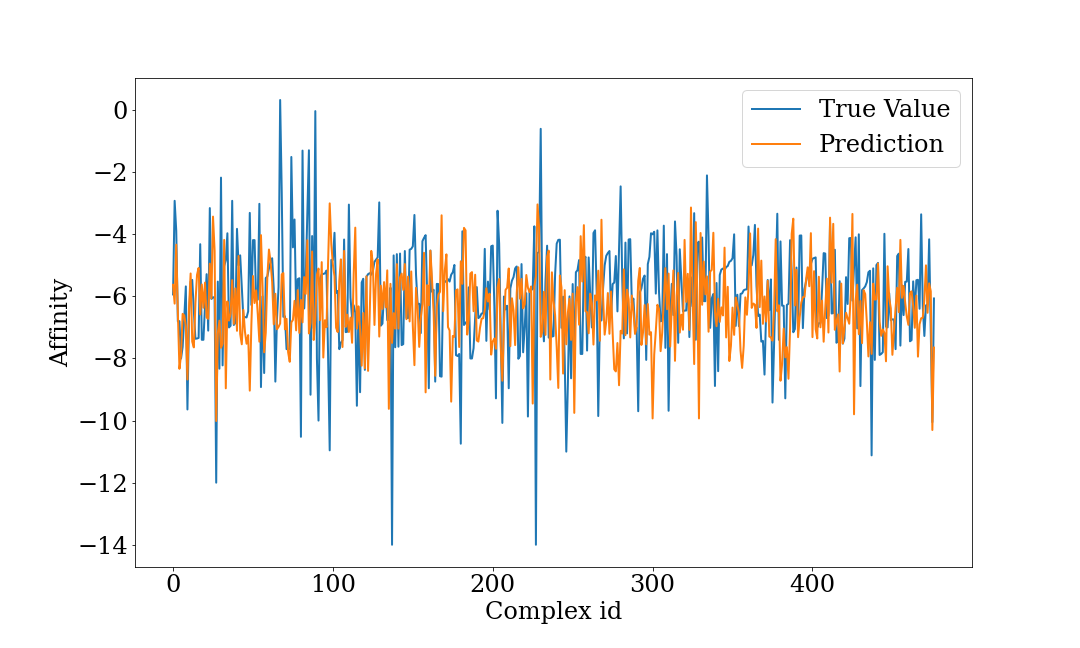
\includegraphics[width=0.8\textwidth]{contents/pred.png}
\end{center}

\begin{center}
\caption{Base CatBoost model errors}
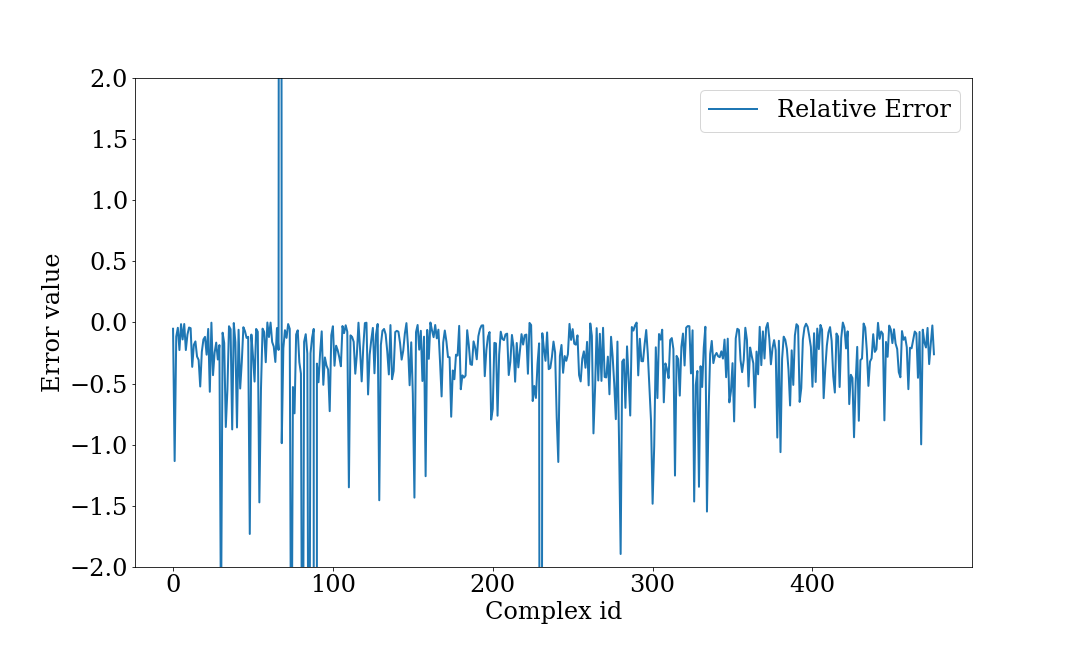
\includegraphics[width=0.8\textwidth]{contents/error.png}
\end{center}

\href{https://catboost.ai/docs/concepts/python-quickstart}{CatBoost} model with default parameters is our base model with MSE of $4.8$. On the figures above one can find a relative error on the test data set and a prediction itself. 
We plan to benchmark our models against existing state-of-the art solutions and this one. Our current suggestions are Graph Neural Network and 3D-CNN.
\section{Experiment Flow}
We fit a model on the train dataset. Optimal parameters are chosen through cross-validation if needed. We analyze model robustness and calculate Mean Squared Error of prediction. \
\subsection{Expected tables and figures}
\begin{enumerate}
    \item Graph of model prediction and true target against complex index
    \item Histogram of relative error distribution
    \item Table with MSE depending on model parameters selection
\end{enumerate}
\subsection{Visualization}
The source dataset contains 2327 protein complexes. We provide following plots for better understanding of given input.
\begin{figure}[!ht]
  \subfloat{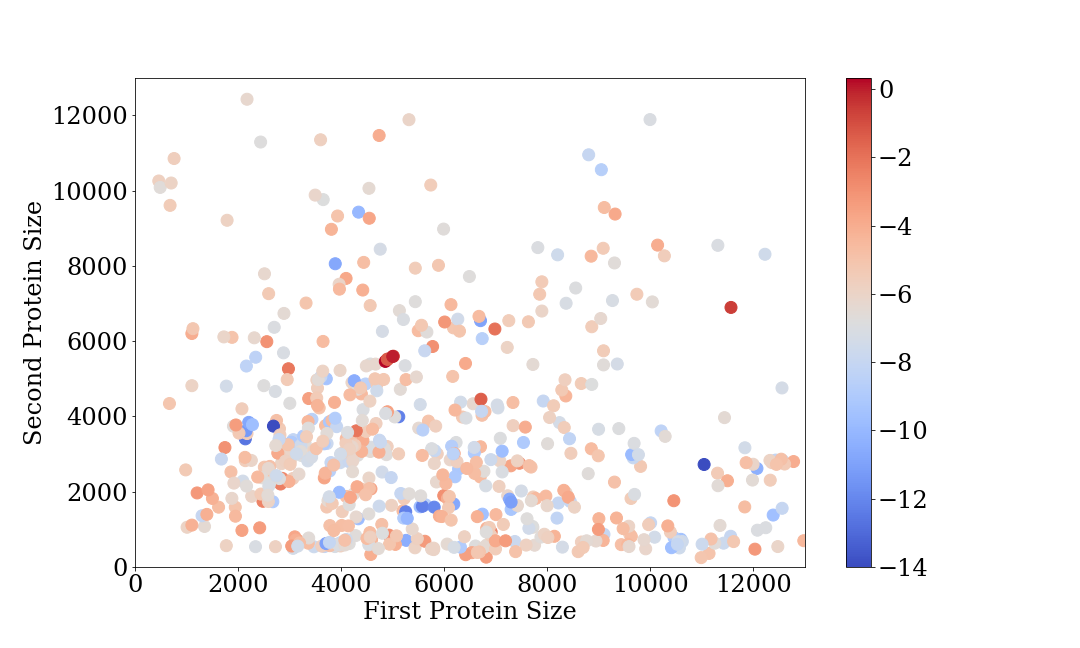
\includegraphics[width=0.5\textwidth]{contents/visual.png}}
  \subfloat{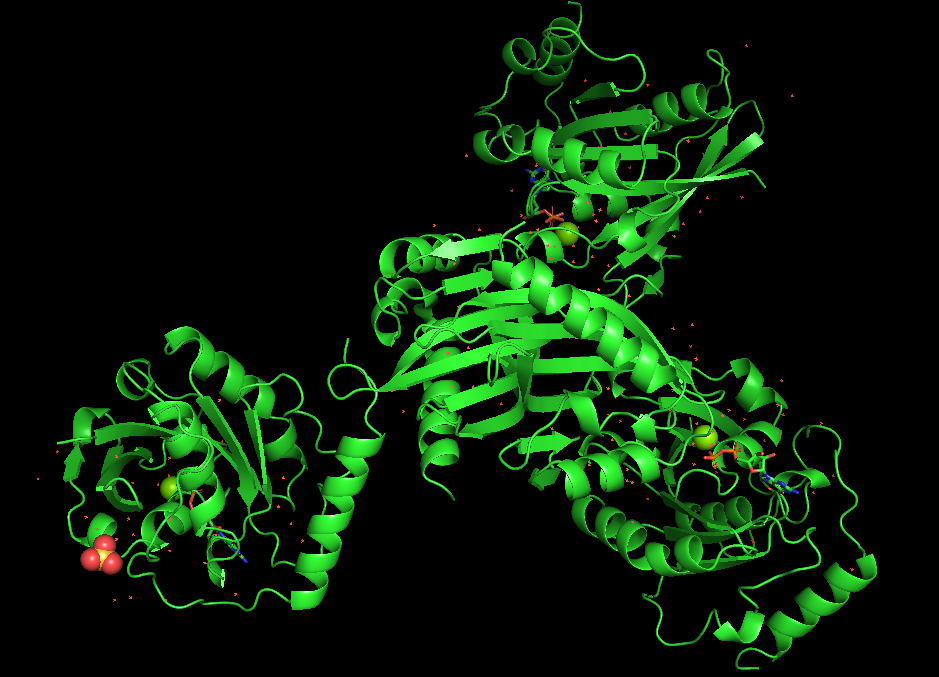
\includegraphics[width=0.5\textwidth]{contents/complex.png}}\\
 \caption{Source data target visualization / Example of source protein}
  \label{fig:3}
\end{figure}
\bibliographystyle{plain} % We choose the "plain" reference style
\bibliography{links} % Entries are in the refs.bib file
\newpage
% \input{contents/listings}
\end{document}